\documentclass[a4paper]{article}

\usepackage[T1]{fontenc}
\usepackage{ucs}
\usepackage[utf8]{inputenc}

\usepackage[a4paper, total={6in, 8in}]{geometry} % Set margins

\usepackage{acronym} % \ac[p], \acl[p], \acs[p], \acf[p]
\usepackage{algorithm} % \begin{algorithm} \end{algorithm}
\usepackage{algpseudocode} % \begin{algorithmic} \end{algorithmic}
\usepackage{amsthm} % \newtheorem
\newtheorem{mydef}{Definition}

\usepackage{color}
\AtBeginDocument{
\definecolor{pdfurlcolor}{rgb}{0,0,0}
\definecolor{pdfcitecolor}{rgb}{0,0,0}
\definecolor{pdflinkcolor}{rgb}{0,0,0}
\definecolor{light}{gray}{.85}
\definecolor{vlight}{gray}{.95}
\definecolor{darkgreen}{rgb}{0.0, 0.2, 0.13}
}
\usepackage[colorlinks=true,
            citecolor=pdfcitecolor,
            urlcolor=pdfurlcolor,
            linkcolor=pdflinkcolor,
            pdfborder={0 0 0}
            ]{hyperref}
\usepackage{url}
\urlstyle{rm}
\usepackage{paralist}
\usepackage{booktabs}
\usepackage{bookmark}

\usepackage{etoolbox}
\usepackage{tikz}
\usetikzlibrary{positioning, shapes}

% Acronyms
% --------
\acrodef{CRDT}[CRDT]{Conflict-free Replicated Data Type}
\acrodefplural{CRDT}[CRDTs]{Conflict-free Replicated Data Types}

% Meta-Data
% ---------
\title{Research report : renaming in Identifier-based Sequence \acfp{CRDT}}
\author{Matthieu Nicolas}

\hypersetup{pdftitle={Research report : renaming in Identifier-based Sequence CRDT},
  pdfsubject={},
  pdfkeywords={Data replication, CRDT},
  pdfauthor={M. Nicolas}}

\clubpenalty=10000
\widowpenalty=10000
\tolerance=1
\emergencystretch=\maxdimen
\hyphenpenalty=10000
\hbadness=10000

\pagestyle{empty}


\newcommand{\numToText}[1]{%
  \ifcase#1\or one\or two\or three\or four\or five\or six\or seven\or eight\or nine\or ten\or
    eleven\or twelve\or thirteen\or fourteen\or fifteen\or sixteen\or seventeen\or eighteen\or nineteen\or twenty\or Lots
  \fi
}

\newcommand{\drawState}[6] {
  % #1: position (node identifier)
  % #2: positioning (below, above)
  % #3: name of state
  % #4: state
  % #5: name of log
  % #6: log entries
  \node[#2=1pt of #1] {#3};
  \node[#2=11pt of #1] {#4};
  \node[#2=30pt of #1] {#5};

  % Generate the content of the log
  \def \logcontents{}
  \foreach[count=\counter] \remote/\local in {#6} {
    \xappto{\logcontents}{
      \noexpand
      \nodepart{\numToText{\counter}}
      $remoteOp_\remote$
    }
  }
  % Draw log
  \node[#2=45pt of #1,
    scale=0.75,
    align=center,
    draw,
    rectangle split,
    rectangle split horizontal,
    rectangle split parts=\counter] {
    \logcontents
  };
}

\begin{document}

\maketitle
\thispagestyle{empty}

\section{Context}

\subsection{System model}

\begin{itemize}
  \item Distributed large-scale system
  \item Asynchronous network
  \item Partition-tolerant
  \item Replicated sequence among nodes
  \item Eventual consistency
  \item Use a Identifier-based Sequence \ac{CRDT} as the conflict resolution mechanism
  \item Intention preserving
\end{itemize}

\subsection{Identifier-based Sequence \acfp{CRDT}}

\subsubsection{State}

Has a state $S$ which represents the replicated sequence (use additional metadata to do so)
\begin{itemize}
  \item Noted as $[(id, elt)]$ in the following figures
  \item The function $view(S)$ allows to retrieve the sequence represented by the state $S$
  \item \textbf{Example:} $view([(id_1, elt_1), (id_2, elt_2)]) = [elt_1, elt_2]$
\end{itemize}

\subsubsection{Identifiers}

\paragraph{Description} ~\\

Associates an identifier $id$ to each element $elt$ of the sequence
\begin{itemize}
  \item Unique (an identifier can not be generated twice)
  \item Order relation (so that we can compare two identifiers)
  \begin{itemize}
    \item Allows to determine the order of elements of the sequence using their identifiers
  \end{itemize}
  \item Belong to a dense set
  \begin{itemize}
    \item Always able to add a new element (and thus a new identifier) between two other elements
  \end{itemize}
\end{itemize}

The elements in the sequence are always ordered according to their identifiers :
in a sequence $[(id_1, elt_1), ..., (id_3, elt_3), ..., (id_2, elt_2)]$
we always have $id_1 < ... < id_3 < ... < id_2$.

\paragraph{Details} ~\\

An identifier is actually composed of a list of tuples. Each tuple is of the following form:
\begin{center}
$<pos, id_{site}, clock_{site}>$
\end{center}
where
\begin{itemize}
  \item $pos: Int$, allows to determine the position of this identifier compare to other ones.
  \item $id_{site}: Int$, refers to the site's identifier, assumed to be unique.
  \item $clock_{site}: Int$, refers to the site's logical clock, which increases monotically with local operations.
\end{itemize}

We note the $id_{site}$ and the $clock_{site}$ of the last tuple of $id$
as $id.id_{site}$ and $id.clock_{site}$ respectively.
\paragraph{Generation} ~\\

To generate a new identifier $id_3$ between two others
$id_1 = [tuple_{1,1}, tuple_{1,2},...,tuple_{1,n}]$ and
$id_2 = [tuple_{2,1}, tuple_{2,2},...,tuple_{2,n}]$,
we use the algorithm \ref{alg:generate-id}:


\begin{algorithm}
  \caption{Identifier generation algorithm (simplified)}\label{alg:generate-id}
  \begin{algorithmic}
    \Function{generateIdentifier}{$id_1: Id, id_2: Id, id_{site}: Int, clock_{site}: Int$}{$:Id$}
      \Require $id_1 < id_2$
      \Ensure $id_1 < id_3 < id_2$
      \Statex
      \State $id_3 \gets [~]$
      \State $continue \gets true$
      \State $i \gets 0$
      \While{$continue$}
        \State $tuple_1 \gets id_1[i]$
        \State $tuple_2 \gets id_2[i]$
        \If{$tuple_2.pos - tuple_1.pos > 2$}
          \State $newPos \gets randomBetween(tuple_1.pos, tuple_2.pos)$
          \State $id_3 \gets id_3 :: <newPos, id_{site}, clock_{site}>$
          \State $continue \gets false$
        \Else
          \State $id_3 \gets id_3 :: tuple_1$
        \EndIf
        \State $i \gets i+1$
      \EndWhile
      \State \Return $id_3$
    \EndFunction
  \end{algorithmic}
\end{algorithm}


We compare the identifiers' tuples in a pairwise manner.
As soon as we are able to generate a new tuple $tuple_3$ such as $tuple_1 < tuple_3 < tuple_2$,
we add it to $id_3$ and return the later.
\\
If we can not generate such a tuple,
we add instead $tuple_1$ to $id_3$ and move to the next pair.
\\
\textbf{Note:} If the identifiers $id_1$ and $id_2$ have different sizes,
we use some default tuples to "fill" the shorter of the two:
\begin{itemize}
  \item $minTuple$ if it is $id_1$
  \item $maxTuple$ otherwise
\end{itemize}

\paragraph{Comparison} ~\\

To compare two identifiers, we use the algorithm \ref{alg:compare-ids}:

\begin{algorithm}
  \caption{Identifier comparison algorithm}\label{alg:compare-ids}
  \begin{algorithmic}
    \Function{compareIdentifiers}{$id_1: Id, id_2: Id$}{$: LESS~|~EQUALS~|~GREATER$}
      \For{$i \gets 0, min(id_1.length, id_2.length)$}
        \State $tuple_1 \gets id_1[i]$
        \State $tuple_2 \gets id_2[i]$
        \If{$tuple_1.pos < tuple_2.pos$}
          \State \Return $LESS$
        \ElsIf{$tuple_1.pos > tuple_2.pos$}
          \State \Return $GREATER$
        \ElsIf{$tuple_1.id_{site} < tuple_2.id_{site}$}
          \State \Return $LESS$
        \ElsIf{$tuple_1.id_{site} > tuple_2.id_{site}$}
          \State \Return $GREATER$
        \ElsIf{$tuple_1.clock_{site} < tuple_2.clock_{site}$}
          \State \Return $LESS$
        \ElsIf{$tuple_1.clock_{site} > tuple_2.clock_{site}$}
          \State \Return $GREATER$
        \EndIf
      \EndFor
      \If{$id_1.length < id_2.length$}
        \State \Return $LESS$
      \ElsIf{$id_1.length > id_2.length$}
        \State \Return $GREATER$
      \EndIf
      \State \Return $EQUALS$
    \EndFunction
  \end{algorithmic}
\end{algorithm}

When comparing two identifiers, we compare theirs tuples in a pairwise manner.
As soon as we find one element which is different from its pair,
we can determine the order between the two identifiers.

\subsubsection{Operations}

For each operation to update the data structure, has two forms of it: the $local$ form and the $remote$ one
\begin{itemize}
  \item The $local$ operation is triggered by the node (by user request for example)
  \item Performing a $local$ operation on a given state $S$
    returns the new state $S'$ and the metadata needed to build an equivalent $remote$ operation
  \item The $remote$ operation is propagated to other nodes so they can also update their own state
  \item Given a state $S$ and an operation $localOp(S, data) = (S', metadata)$, we have $remoteOp(S, metadata) = S'$
  \item \textbf{Note: } given an $local$ operation $localOp$, there may be several equivalent $remote$ operations $remoteOp$, $remoteOp'$, $remoteOp"$...
\end{itemize}

We note the identifier of the element targeted by a $remote$ operation as $remoteOp.id$.
\subsubsection{$add$}

The operation $add$ allows to insert an element into the sequence :
\begin{itemize}
  \item $addLocal(S, index, elt) = (S', (id, elt))$
  \begin{itemize}
    \item Update state $S$ by adding an element $elt$ at the position $index$ in the sequence
    \item Return the resulting state $S'$ as well as the identifier $id$ generated for this element
    \item The identifier $id$ will be generated according to the identifiers of the elements previously at the positions $index-1$ and $index$
    \begin{itemize}
      \item \textbf{Example: } $addLocal([(id_1, elt_1), (id_2, elt_2)], 1, elt_3)$ will return $id_3$\\ such as $id_1 < id_3 < id_2$
    \end{itemize}
    \item This identifier $id$ will be used (and especially its order relation with other identifiers) to update correctly other nodes' state
    \item \textbf{Note: } When generating a new identifier between $id_1$ and $id_2$,
      there may be several identifiers $id_3$, $id_3'$, $id_3"$... such as
      $id_1 < id_3 < id_3' < id_3" < id_2$. The returned identifier is chosen in a undeterministic manner.
  \end{itemize}
  \item $addRemote(S, id, elt) = (S', (index, elt))$
  \begin{itemize}
    \item Update state $S$ by adding an element $elt$ in the sequence
    \item The position of insertion of this element will be determined using its $id$
    \item Return the resulting state $S'$ as well as the current index of the element in the sequence
  \end{itemize}
  \item Given a state $S$, to one $addLocal$ operation on $S$, many $addRemote$ correspond
    (since the resulting $id$ is generated in an undeterministic manner)
  \item Given a state $S$, to one $addRemote$ operation on $S$, only one $addLocal$ corresponds
\end{itemize}

\subsubsection{$del$}

The operation $del$ allows to remove an element from the sequence :
\begin{itemize}
  \item $delLocal(S, index) = (S', id)$
  \begin{itemize}
    \item Update state $S$ by removing the element at the position $index$ in the sequence
    \item Return the resulting state $S'$ as well as the identifier $id$ of the deleted element
  \end{itemize}
  \item $delRemote(S, id) = (S', index)$ allowing to remove the element identified by $id$
  \begin{itemize}
    \item Update state $S$ by removing the element identified by $id$
    \item Return the resulting state $S'$ as well as the position $index$ of the deleted element in the sequence
  \end{itemize}
  \item Given a state $S$, to one $delLocal$ operation, only one $delRemote$ corresponds
  \item Given a state $S$, to one $delRemote$ operation, only one $delLocal$ corresponds
\end{itemize}

\subsubsection{Log of operations}

Associates to a state $S$ a log $L$
\begin{itemize}
  \item Is a sequence of the $remote$ operations observed
  \item The sequence of remote operations,
    performed in order from a blank state $S_{blank}$,
    allows to recreate state $S$
  \item Each entry is represented as
    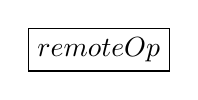
\begin{tikzpicture}
      \node[draw, rectangle, align=center] {$remoteOp$};
    \end{tikzpicture} in the following figures
\end{itemize}

\subsubsection{Causal context}

Associates to a state $S$ a causal context $cc$
\begin{itemize}
  \item Represents all operations known at state $S$
  \item Can use a \emph{version vector} for example as an implementation
\end{itemize}

An example of the lifecycle of such a replicated data structure is shown in figure~\ref{inserts}

\begin{figure}[h]
  \begin{tikzpicture}[
    localOp/.style={->, thick, shorten <=3pt, shorten >=3pt},
    remoteOp/.style={->, dotted, thick, shorten <=3pt, shorten >=3pt},
    trait/.style={fill, rectangle, xscale=0.1},
    medium/.style={scale=0.85}]

    \newcommand{\sOne}{$[(id_1, elt_1)]$}
    \newcommand{\sTwo}{$[(id_1, elt_1), (id_2, elt_2)]$}
    \newcommand{\sThree}{$[(id_1, elt_1), (id_3, elt_3), (id_2, elt_2)]$}

    \node (A) at (0, 0) {node A};
    \node[right=5pt of A] (beginA) {};
    \node[trait, right=of beginA] (S1A) {};
    \drawState{S1A}{above}{$S_1$}{\sOne}{$L_1$}{1/1}
    \node[trait, right=5 of A] (S2A) {};
    \drawState{S2A}{above}{$S_2$}{\sTwo}{$L_2$}{1/1, 2/2}
    \node[right=14 of A] (endA) {};

    \node (B) at (0, -2) {node B};
    \node[right=5pt of B] (beginB) {};
    \node[trait, right=of beginB] (S1B) {};
    \drawState{S1B}{below}{$S_1$}{\sOne}{$L_1$}{1/1}
    \node[trait, right=7 of B] (S2B) {};
    \drawState{S2B}{below}{$S_2$}{\sTwo}{$L_2$}{1/1, 2/2}
    \node[trait, right=6 of S2B] (S3B) {};
    \drawState{S3B}{below}{$S_3$}{\sThree}{$L_3$}{1/1, 2/2, 3/3}
    \node[right=14 of B] (endB) {};

    \draw[->] (beginA) -- (endA);
    \draw[->] (beginB) -- (endB);
    \draw[localOp] (S1A) to[out=-15, in=195] node[below, medium] {$localOp_2=addLocal(1, elt_2)$} (S2A);
    \draw[remoteOp] (S2A) -- node[near start, right, xshift=5pt, medium] {$remoteOp_2=addRemote(id_2, elt_2)$} (S2B);
    \draw[localOp] (S2B) to[out=15, in=165] node[above, medium] {$localOp_3=addLocal(1, elt_3)$} (S3B);

  \end{tikzpicture}
  \caption{Insertion of elements in the replicated sequence}
  \label{inserts}
\end{figure}

\section{$rename$ operations}

\subsection{Motivation}

\begin{itemize}
  \item Identifiers growing over time
  \item Performances of the data structure thus decreasing over time
\end{itemize}

\subsection{$renameLocal$}

\paragraph{Definition}~\\

\begin{itemize}
  \item Add an operation $renameLocal(S) = (S', mapIds, cc_S)$
  \begin{itemize}
    \item Replace each identifier attached to elements of $S$ with new ones
    \item Return a map $mapIds$ of the previous identifiers to the new ones
    \item Also need to return the causal context $cc_S$ of the state $S$
      to indicate on which state has been performed the renaming operation
    \item $view(S) = view(S')$ where $(S', \_, \_) = renameLocal(S)$
  \end{itemize}
\end{itemize}

\subsection{$renameRemote$}

\begin{itemize}
  \item Add an operation $renameRemote(S, L, mapIds, cc_{S'}) = (S", L")$
  \begin{itemize}
    \item Replace current state $S$ by equivalent state $S"$ and current log $L$ by equivalent log $L"$
    \item Rename all identifiers $id \in S \cdot id \in S'$ using $mapIds$
    \item Also have to rename all identifiers $id \in S \cdot id \notin S'$ to preserve the current order of elements
    \item \textbf{Precondition: } $S \geq S'$ ($S$ has seen all the operations seen by $S'$ but may have seen more)
    \item $view(S) = view(S")$ where $(S", \_) = renameRemote(S, L, mapIds, cc_{S'})$
  \end{itemize}
\end{itemize}

\subsection{Usage}
\label{sec:usage}

Given an operation $renameRemote(S, L, mapIds, cc_{S'})$,
resulting from the execution of $renameLocal(S')$ on another node,
we have to perform the following steps to apply it:

\begin{enumerate}
  \item Instantiate a blank state $S"$ and its empty log $L"$
  \item Generate a log $L_{causal}$
    made of all operations belonging to the causal context $cc_{S'}$
  \item For each entry $(remoteOp, localOp)$ of $L_{causal}$
  \begin{enumerate}
    \item Update state $S"$ by performing  $remoteOp(S", metadata)$
    \item Add entry $(remoteOp, localOp)$ to $L"$
  \end{enumerate}
  \item Rename all identifiers of the data structure according to $mapIds$ (at this point, $S" = S'$)
  \item Generate a log $L_{concurrent}$ made of all operations of $L$ not included in $L_{causal}$
  \item For each entry $(remoteOp, localOp)$ of $L_{concurrent}$
  \begin{enumerate}
    \item Update state $S"$ by performing $localOp(S"_{prev}) = (S"_{new}, metadata)$
    \label{itm:replay-local-op}
    \item Build new remote operation $remoteOp'$ given $metadata$
    \label{itm:regenerate-remote-op}
    \item Add entry $(remoteOp', localOp)$ to $L"$
    \item Propagate $remoteOp'$
  \end{enumerate}
\end{enumerate}

This algorithm is represented by figure~\ref{renameRemote}

\begin{figure}[h]
  \begin{tikzpicture}[
    localOp/.style={->, thick, shorten <=3pt, shorten >=3pt},
    remoteOp/.style={->, dotted, thick, shorten <=3pt, shorten >=3pt},
    trait/.style={fill, rectangle, xscale=0.1},
    medium/.style={scale=0.85}]

    \newcommand{\sTwo}{$[(id_1, elt_1), (id_2, elt_2)]$}
    \newcommand{\sThree}{$[(id_1, elt_1), (id_3, elt_3), (id_2, elt_2)]$}
    \newcommand{\sFour}{$[(id'_1, elt_1), (id'_2, elt_2)]$}
    \newcommand{\sFive}{$[(id'_1, elt_1), (id'_3, elt_3), (id'_2, elt_2)]$}

    \node (A) at (0, 0) {node A};
    \node[right=5pt of A] (beginA) {};
    \node[trait, right=of beginA] (S4A) {};
    \drawState{S4A}{above}{$S_4$}{\sFour}{$L_4$}{1/1, 2/2, 4/4}
    \node[right=13 of A] (endA) {};

    \node (B) at (0, -2) {node B};
    \node[right=5pt of B] (beginB) {};
    \node[trait, right=of beginB] (S3B) {};
    \drawState{S3B}{below}{$S_3$}{\sThree}{$L_3$}{1/1, 2/2, 3/3}
    \node[trait, right=6 of S3B] (receivedOp4B) {};
    \node[right=13 of B] (endB) {};

    \node[align=center] (zoomB) at (0, -8) {zoom on \\node B};
    \node[right=5pt of zoomB] (beginZoomB) {};
    \node[trait, right=of beginZoomB] (SBlank) {};
    \node[below=1pt of SBlank] {$S_{blank}$};
    \node[trait, right=4 of SBlank] (S4B) {};
    \drawState{S4B}{below}{$S_4$}{\sFour}{$L_4$}{1/1, 2/2, 4/4};
    \node[trait, right=7 of S4B] (S5B) {};
    \drawState{S5B}{below}{$S_5$}{\sFive}{$L_5$}{1/1, 2/2, 4/4, 3'/3}
    \node[right=14 of zoomB] (endZoomB) {};

    \draw[->] (beginA) -- (endA);
    \draw[->] (beginB) -- (endB);
    \draw[->] (beginZoomB) -- (endZoomB);
    \draw[->, dotted] (receivedOp4B) -- (beginZoomB);
    \draw[->, dotted, shorten >=3pt] (endZoomB) -- (receivedOp4B);
    \draw[remoteOp] (S4A) -- node[near start, right, xshift=10pt, medium] {$remoteOp_4=renameRemote(id_1 \rightarrow id_1', id_2 \rightarrow id_2', cc_{S_2})$} (receivedOp4B);
    \draw[localOp] (SBlank) to[out=15, in=165] node[above, medium, align=center] {$remoteOp_1$\\$remoteOp_2$\\$remoteOp_4$} (S4B);
    \draw[localOp] (S4B) to[out=15, in=165] node[above, medium] {$localOp_3$} (S5B);

  \end{tikzpicture}
  \caption{Renaming with concurrent operations}
  \label{renameRemote}
\end{figure}

\subsection{Limits}

\begin{itemize}
  \item Differents nodes, while performing the remote renaming operation,
    may replay at step \ref{itm:replay-local-op} the same operation
  \item Since there is no coordination between them, in the case of a $addLocal$,
    they will end up generating two different remote operations
    $remoteOp'$ and $remoteOp"$ during step \ref{itm:regenerate-remote-op}
  \item We will have to deliver them both to each node to actually converge
    (the states would differ otherwise)
  \item This will result in the duplication of the user's intention
    (since the inserted element will end up being added twice)
  \item An example is show in figure~\ref{intention-duplication}
\end{itemize}

\begin{figure}[h]
  \begin{tikzpicture}[
    localOp/.style={->, thick, shorten <=3pt, shorten >=3pt},
    remoteOp/.style={->, dotted, thick, shorten <=3pt, shorten >=3pt},
    trait/.style={fill, rectangle, xscale=0.1},
    medium/.style={scale=0.85}]

    \newcommand{\sThree}{$[(id_1, elt_1), (id_3, elt_3), (id_2, elt_2)]$}
    \newcommand{\sFour}{$[(id'_1, elt_1), (id'_2, elt_2)]$}
    \newcommand{\sFive}{$[(id'_1, elt_1), (id'_3, elt_3), (id'_2, elt_2)]$}
    \newcommand{\sSix}{$[(id'_1, elt_1), (id"_3, elt_3), (id'_2, elt_2)]$}
    \newcommand{\sSeven}{$[(id'_1, elt_1), (id'_3, elt_3), (id"_3, elt_3), (id'_2, elt_2)]$}

    \node (A) at (0, -2) {node A};
    \node[right=5pt of A] (beginA) {};
    \node[trait, right=of beginA] (S4A) {};
    \node[below=1pt of S4A] {$S4$};
    \node[trait, right=11 of A] (S7A) {};
    \node[below=1pt of S7A] {$S7$};
    \node[right=14 of A] (endA) {};

    \node (B) at (0, 0) {node B};
    \node[right=5pt of B] (beginB) {};
    \node[trait, right=of beginB] (S3B) {};
    \node[above=1pt of S3B] {$S3$};
    \node[trait, right=3 of B] (S5B) {};
    \node[above=1pt of S5B] {$S5$};
    \node[trait, right=8 of S5B] (S7B) {};
    \drawState{S7B}{above}{$S_7$}{\sSeven}{$L_7$}{1/1, 2/2, 4/4, 3'/3, 3"/3};
    \node[right=14 of B] (endB) {};

    \node (C) at (0, -4) {node C};
    \node[right=5pt of C] (beginC) {};
    \node[trait, right=of beginC] (S3C) {};
    \node[above=1pt of S3C] {$S3$};
    \node[trait, right=3 of C] (S6C) {};
    \drawState{S6C}{below}{$S_6$}{\sSix}{$L_6$}{1/1, 2/2, 4/4, 3"/3};
    \node[trait, right=8 of S6C] (S7C) {};
    \drawState{S7C}{below}{$S_7$}{\sSeven}{$L'_7$}{1/1, 2/2, 4/4, 3"/3, 3'/3};
    \node[right=14 of C] (endC) {};

    \draw[->] (beginA) -- (endA);
    \draw[->] (beginB) -- (endB);
    \draw[->] (beginC) -- (endC);
    \draw[remoteOp] (S4A) -- node[near start, right, xshift=5pt, medium] {$remoteOp_4$} (S5B);
    \draw[remoteOp] (S4A) -- node[near start, right, xshift=5pt, medium] {$remoteOp_4$} (S6C);
    \draw[remoteOp] (S5B) -- node[near start, right, xshift=10pt, yshift=5pt, medium] {$remoteOp_3'$} (S7A);
    \draw[remoteOp] (S5B) -- (S7C);
    \draw[remoteOp] (S6C) -- node[near start, right, xshift=10pt, yshift=-5pt, medium] {$remoteOp_3"$} (S7A);
    \draw[remoteOp] (S6C) -- (S7B);

  \end{tikzpicture}
  \caption{Duplication of the intention of $localOp_3$}
  \label{intention-duplication}
\end{figure}

\section{$addRedo$ operation}

\subsection{Idea}

\begin{itemize}
  \item At step \ref{itm:replay-local-op}, if we can generate deterministically the resulting $id$
    for a given previous log entry $(addRemote, addLocal)$, then we would not duplicate the user's intention
  \item Indeed, each node would thus generates the same operation $addRemote'$ at step \ref{itm:regenerate-remote-op}
  \item In that case, we would only need to deliver at least once $addRemote'$ to the nodes to converge
    (or exactly-once if the $addRemote$ is not idempotent)
\end{itemize}

\subsection{Research question}

Can we define the following operation $addRedo(S, (addRemote, addLocal)) = (S', (id', elt))$ such as :
\begin{itemize}
  \item $id'$ is generated deterministically
  \item $view(S) = view(S')$
    where $(S, id) = addLocal(S", index, elt)$
    and $(S', \_) = addRedo(S", (addRemote(S", id, elt), addLocal(S", index, elt))$
\end{itemize}
This operation would be used at step \ref{itm:replay-local-op} instead of simply using $addLocal$
and would solve the duplication effect.

\section{Discussion}

\begin{itemize}
  \item Need to keep the log of operations (both $remote$ and $local$)
  \item Performances of a $renameRemote$ depend on the number of operations in the log and the number of concurrent operations
  \begin{itemize}
    \item Have to replay all operations from the causal context of the $renameRemote$ operation
    \item Have to regenerate concurrent operations and propagate them
  \end{itemize}
  \item Can propose mechanism to reduce the size of the log
  \begin{itemize}
    \item By pruning causally stable entries and using snapshots
  \end{itemize}
  \item New identifiers generated by $addRedo$ operations may be larger than the initial ones according to the chosen strategy
  \begin{itemize}
    \item Can argue that they will shrink with the next $rename$
  \end{itemize}
  \item Solving concurrent $rename$ looks difficult
  \begin{itemize}
    \item For now, can assume that only one node can perform such operations
  \end{itemize}
\end{itemize}

\section{Counter-example}

Found a counter-example which invalidate the algorithm proposed in section \ref{sec:usage}.
We replay the same operations as in previous examples but in this case:
\begin{itemize}
  \item $localOp_2$ and $localOp_3$ are concurrent
  \item The generated identifiers $id_2$ and $id_3$ are in this order: $id_2 < id_3$
\end{itemize}
In this scenario, when replaying $localOp_3$ at step \ref{itm:replay-local-op},
we will swap the position of the elements $elt_2$ and $elt_3$
compared to the previously observed state.
This result in a incoherence of the system and may result in the violation
of the intention of following operations based on this previously observed state.
This scenario is represented by figure \ref{fig:incoherent-replay-local-op}.

\begin{figure}[h]
  \begin{tikzpicture}[
    localOp/.style={->, thick, shorten <=3pt, shorten >=3pt},
    remoteOp/.style={->, dotted, thick, shorten <=3pt, shorten >=3pt},
    trait/.style={fill, rectangle, xscale=0.1},
    medium/.style={scale=0.85}]

    \newcommand{\sOne}{$[(id_1, elt_1)]$}
    \newcommand{\sTwo}{$[(id_1, elt_1), (id_2, elt_2)]$}
    \newcommand{\sThree}{$[(id_1, elt_1), (id_3, elt_3)]$}
    \newcommand{\sFour}{$[(id'_1, elt_1), (id'_2, elt_2)]$}
    \newcommand{\sFive}{$[(id_1, elt_1), (id_2, elt_2), (id_3, elt_3)]$}
    \newcommand{\sSix}{$[(id'_1, elt_1), (id'_3, elt_3), (id'_2, elt_2)]$}

    \node (A) at (0, 0) {node A};
    \node[right=5pt of A] (beginA) {};
    \node[trait, right=of beginA] (S1A) {};
    \drawState{S1A}{above}{$S_1$}{\sOne}{$L_1$}{1/1};
    \node[trait, right=3 of S1A] (S2A) {};
    \drawState{S2A}{above}{$S_2$}{\sTwo}{$L_2$}{1/1, 2/2};
    \node[trait, right=7 of S2A] (S4A) {};
    \drawState{S4A}{above}{$S_4$}{\sFour}{$L_4$}{1/1, 2/2, 4/4};
    \node[right=15 of A] (endA) {};

    \node (B) at (0, -3) {node B};
    \node[right=5pt of B] (beginB) {};
    \node[trait, right=of beginB] (S1B) {};
    \node[below=1pt of S1B] {$S_1$};
    \node[trait, right=3 of S1B] (S3B) {};
    \node[below=1pt of S3B] {$S_3$};
    \node[trait, right=3 of S3B] (S5B) {};
    \drawState{S5B}{below}{$S_5$}{\sFive}{$L_5$}{1/1, 3/3, 2/2}
    \node[trait, right=7 of S5B] (receivedOp4B) {};
    \node[right=15 of B] (endB) {};

    \node[align=center] (zoomB) at (0, -9) {zoom on \\node B};
    \node[right=5pt of zoomB] (beginZoomB) {};
    \node[trait, right=of beginZoomB] (SBlank) {};
    \node[below=1pt of SBlank] {$S_{blank}$};
    \node[trait, right=4 of SBlank] (S4B) {};
    \drawState{S4B}{below}{$S_4$}{\sFour}{$L_4$}{1/1, 2/2, 4/4};
    \node[trait, right=7 of S4B] (S6B) {};
    \drawState{S6B}{below}{$S_6$}{\sSix}{$L_6$}{1/1, 2/2, 4/4, 3'/3}
    \node[right=15 of beginZoomB] (endZoomB) {};

    \draw[->] (beginA) -- (endA);
    \draw[->] (beginB) -- (endB);
    \draw[->] (beginZoomB) -- (endZoomB);
    \draw[localOp] (S1A) to[out=-15, in=195] node[below, medium, align=center] {$localOp_2=$\\$addLocal(1, elt_2)$} (S2A);
    \draw[localOp] (S2A) to[out=-15, in=195] node[below, medium, xshift=25pt, align=center] {$localOp_4=$\\$renameLocal(id_1 \rightarrow id'_1, id_2 \rightarrow id'_2)$} (S4A);

    \draw[localOp] (S1B) to[out=15, in=165] node[above, medium] {$localOp_3 = addLocal(1, elt_3)$} (S3B);
    \draw[->, dotted] (receivedOp4B) -- (beginZoomB);
    \draw[->, dotted, shorten >=3pt] (endZoomB) -- (receivedOp4B);
    \draw[remoteOp] (S2A) -- node[near end, right, xshift=10pt, medium] {$remoteOp_2$} (S5B);
    \draw[remoteOp] (S4A) -- node[near end, right, xshift=10pt, medium] {$remoteOp_4$} (receivedOp4B);
    \draw[localOp] (SBlank) to[out=15, in=165] node[above, medium, align=center] {$remoteOp_1$\\$remoteOp_2$\\$remoteOp_4$} (S4B);
    \draw[localOp] (S4B) to[out=15, in=165] node[above, medium] {$localOp_3$} (S6B);

  \end{tikzpicture}
  \caption{Incoherence occuring by replaying local operations during renaming process}
  \label{fig:incoherent-replay-local-op}
\end{figure}

\bibliography{ref-selected}

\end{document}
